\begin{figure}[t]
\centering
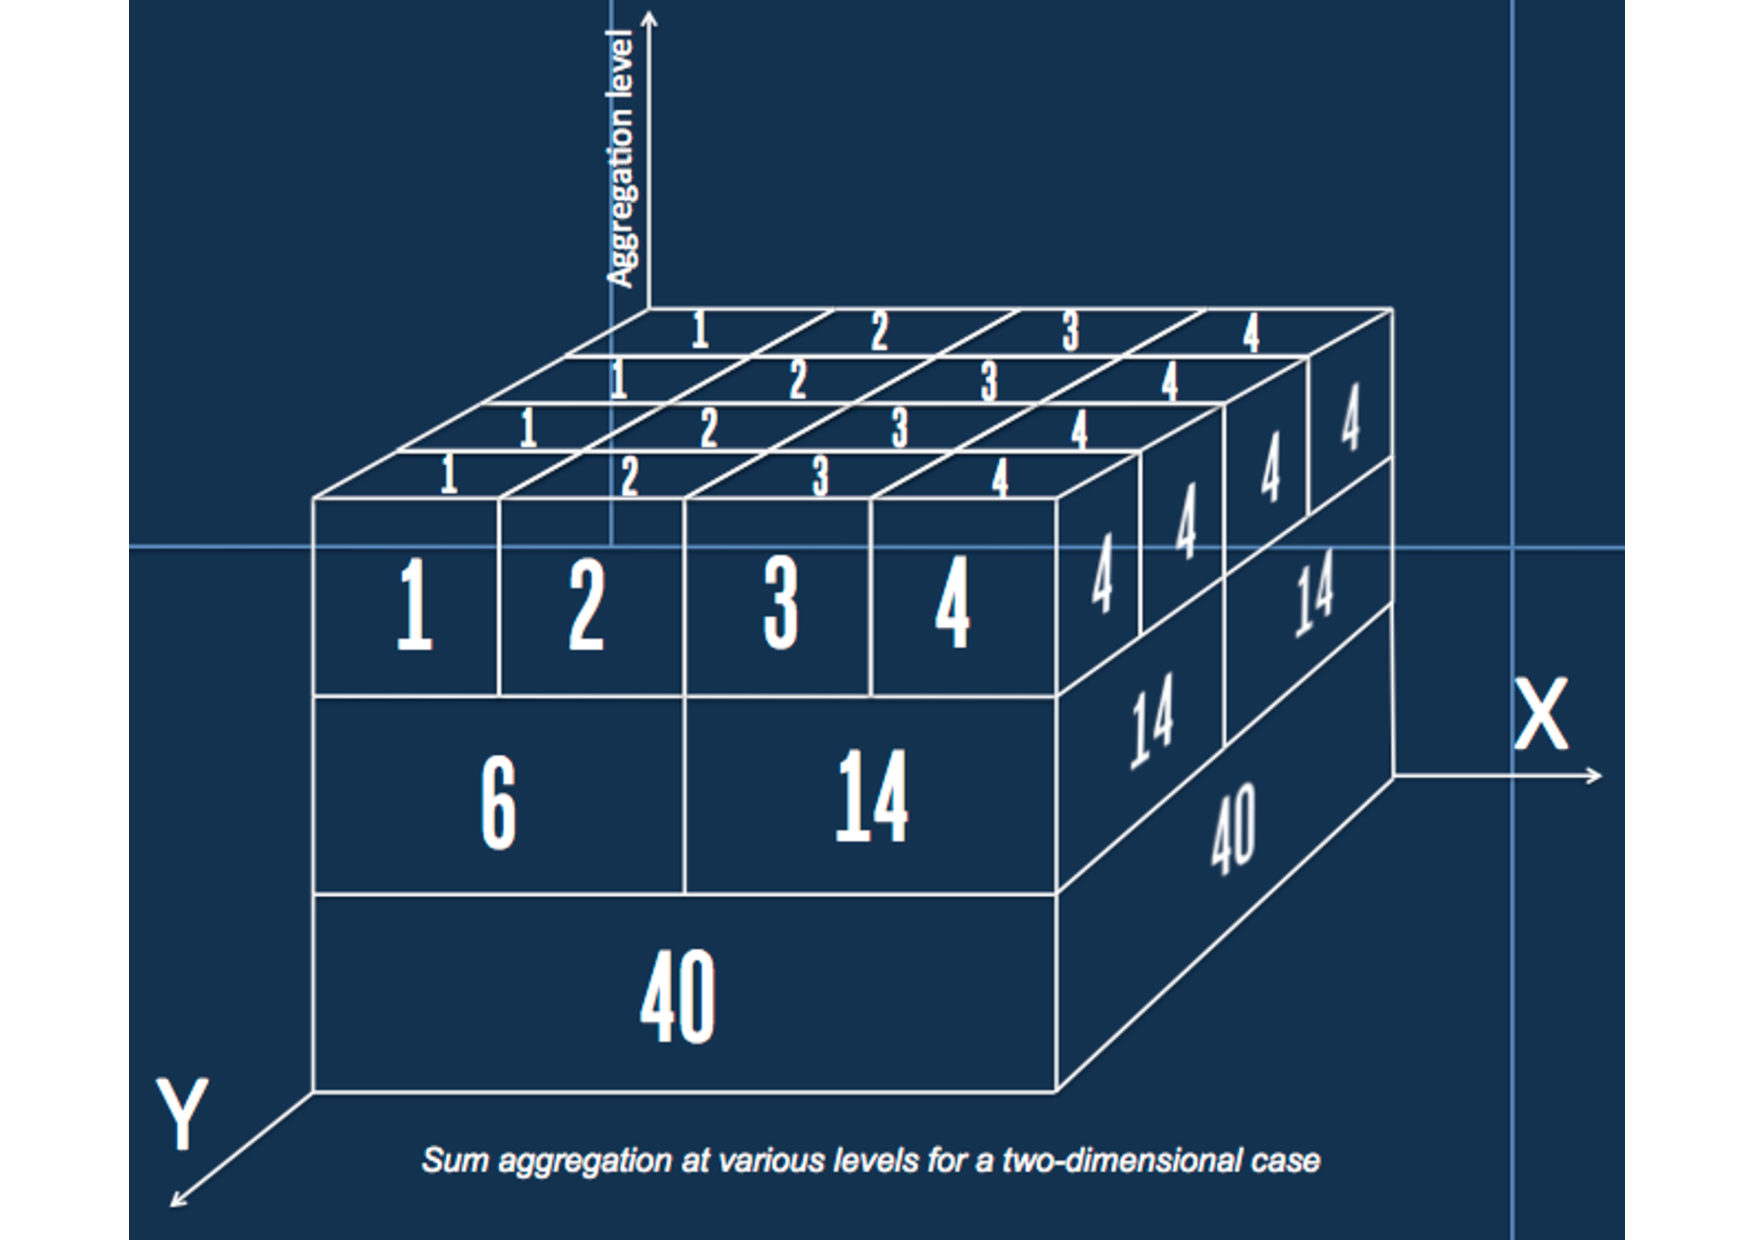
\includegraphics[width=4in]{Figures/grids.pdf}
\caption{Illustration of the grids concept}
\label{fig:grids}
\end{figure}


\subsubsection{Description of Process}

The indexing principle is as follows.  For the indexing of the data,
several grids are defined, with varying grid sizes. These grids can have
any number of dimensions. In the illustration of Figure~\ref{fig:grids}, we
show an example for the two-dimensional case. The third dimension in the
illustration depicts the aggregation grids at the various levels. For each
grid cell, the aggregation function is pre-calculated. Any suitable
aggregation function can be used, such as a summation, count,
maximum/minimum, etc. When a request comes in, the index returns the
pre-calculated values for all entirely included cells. The relatively small
amount of non-indexed values to complete the area is the calculated
on-the-fly, as illustrated on the right.

Concretely, take the dataset of tweets sent within the Netherlands (see
Figure~\ref{fig:NL-screenshot}. A pre-aggregation of this data, i.e.,
counts of tweets, could be in the following form. Dimensions are the x- and
y-coordinate dimensions. We set a highest granularity (zoom-level). The
pre-aggregate algorithm creates blocks bounded by the x- and y-coordinates
at the highest granularity and for all those blocks calculates the number
of tweets within the bounding box. Each subsequent layer is built up from
the previous layer. The final result is a dataset which contains the number
of tweets in a all bounding boxes at all levels of granularity.

\subsubsection{PreAggregate Tool}
\label{sec:preaggtool}

For off-line creation of the pre-aggregation index, a tool has been
developed. The tool can be found in the directory
\lstinline|neogeo/pre-aggregate-tools/|. To generate the binary tools from
source, the Appassembler plugin of Maven is used. Run the following command
to generate the tool.

\begin{lstlisting}
mvn package appassembler:assemble
\end{lstlisting}

After successful completion of this command, a new directory
\lstinline|appassembler| has been created in the \lstinline|target|
directory containing a \lstinline|repo| and a \lstinline|bin| directory.
The \lstinline|bin| directory contains the actual binaries of the tool (in
both Linux/Unix and Windows version) and the \lstinline|repo| directory
contains the tool dependencies. The tool should now be ready for use. An
example of how to compile and use the tool to create a pre-aggregation
index is given in \Fref{sec:examplePreAggIndex}.

The tool is used to create a pre-aggregate index for a table with
$\textit{n}$ dimensions and a measure/aggregate column. It uses with the
following commands:
\begin{lstlisting}[basicstyle=\small]
usage: create-pa-index
 -axistosplit <axis index>    index of axis to split
 -chunksize <size>            maximum chunk size after split
 -config <file>               PreAggregate XML config file
 -d,--database <dbname>       name of database
 -dbtype <postgresql|monetdb> type of database
 -h,--host <host>             database host name or ip address
 -help                        prints this help message
 -p,--port <port>             port number of the database
 -password <password>         database password
 -s,--schema <schema>         schema name in the database
 -u,--user <user>             database username
 -v,--verbose                 Enable verbose output logging
\end{lstlisting}
The tool depends on the \lstinline|PreAggregate.XML| config file which
is used to define the PreAggregate index by specifying the column to
aggregate, the type of aggregate that should done and the dimensions to
include. In the \lstinline|neogeo/pre-aggregate-tools/| directory a sample
configuration file is included.

%\todo[inline, size=\small]{How does this tool work nominal axis? More preprocessing may be required when first parsing words? Example london\_words or gender\_words}

See~\Fref{sec:PreAggregateDev} for more detail about creating a
pre-aggregate index not using the above tool.

Apart from creating a new pre-aggregate index table
\lstinline|<original-table-name>_pa|, pre-aggregation also creates/updates
two other tables: \lstinline|pre_aggregate| and
\lstinline|pre_aggregate_axis|. These two tables are support tables for the
aggregation. They contain information about which tables have been
aggregated and which axis have been used in pre-aggregation.

\subsubsection{Current Status Support of Axis Types}

The dimensions are referred to in the code as \lstinline|AggregateAxis|.
The axes have a base size and all layers above the base size are built up
by aggregating lower layer blocks. Currently the \lstinline|AggregateAxis|
can be split into two different subtypes. The first is a
\lstinline|MetricAxis| and the second is a \lstinline|NominalAxis|. Each
type will be briefly discussed below with examples of data types.

\paragraph{MetricAxis}
A \lstinline|MetricAxis| is the default axis type, it supports a continuous
data type. Examples of such data types are coordinates and time.

\paragraph{NominalAxis}
A \lstinline|NominalAxis| can be used for non-continuous dimensions. An
example for such a data type is a word filter. A \lstinline|NominalAxis|
can be used to split the data on occurrence of $x$ predefined words. 

For example, if a word filter \lstinline|{dog,cat,mouse,horse,NOFILTER}| is
used and a data block represents some text with the sentance
`\lstinline|it's raining cats and dogs|', then three splits would be made.
One on the word \lstinline|dog|, the second on \lstinline|cat| and the
third on \lstinline|NOFILTER|.

\subsubsection{Current Status Support of Aggregation Types}

Currently there are 4 different aggregation types which can be used. These
are discussed below. Note that there is an \lstinline|ALL| option which
returns all aggregate types in the pre-aggregate index. Furthermore these
types can be used to create other types such as average.

The current options are as follows:
\begin{enumerate}
\item \lstinline|ALL|: 	Returns all the aggregation types mentioned below.
\item \lstinline|COUNT|: Returns the count of items in an aggregate box.
\item \lstinline|SUM|: returns the sum of items in an agrregate box.
	For instance, a sum on the tweet length results in the total amount
	of characters tweeted in an aggregate box.
\item \lstinline|MIN|: Returns the lowest value in an aggregate box.
	With the example of tweet length, it returns the length of the shortest
	tweet in the aggregate box.
\item \lstinline|MAX|: Returns the highest value in an aggregate box.
	With the example of tweet length, it returns the longest tweet in the
	aggregate box.
\end{enumerate}

%\todo[inline, size=\small]{Small note, when using the pre-aggregate tool
%(created by Dennis) for the example \lstinline|ALL| was used as it crashed
%when using \lstinline|COUNT|, this should be looked into.}

It is important to choose the right type in order to get the desired
representation of the data.  To show the total number of tweets in a tile,
one should chose \lstinline|COUNT| as this will returns the total number of
data points in a tile. Whereas if one wants only the highest value in the
data (for example the highest building in an area) then \lstinline|MAX|
should be used.
